\documentclass[10pt,a4paper]{amsart}
\usepackage{amsmath,amssymb,amsthm,graphicx}
\usepackage{amsmath,amssymb,mathtools}
\usepackage{hyperref}
\usepackage{graphicx}
\usepackage{fontspec}
\setmainfont{DejaVu Serif}
\sloppy
\setlength{\emergencystretch}{3em}
\title{Colorful fractional Helly theorems for k-dimensional transversals of fat convex Euclidean and spherical sets}
\author{Attila Jung, Dömötör Pálvölgyi}
\date{doi:10.4230/LIPIcs.SoCG.2025.61; CC BY 4.0}
\begin{document}
\maketitle
\noindent\textit{Editorial scope.} Count jointly the mutually supporting Theorems10 and11. Complete official CC BY4.0 author article is transcribed from publisher HTML, with original mathematical alttext used verbatim and original figure converted directly from SVG to vector PDF. All author proofs, definitions, applications and bibliography retained. No author mathematical text rewritten; downstream direct consequences are not separate tasks.\par\medskip
\noindent\textit{Allowed standard prerequisites (editorial).}\begin{itemize}
\item Fractional/colorful Helly arguments, convexity and spherical geometry. Original author introduction and citations retained; source-specific fatness, projection and joint induction proofs complete.
\end{itemize}\medskip
% BEGIN S1
\par\medskip\noindent\textbf{1 Introduction}\par
% BEGIN S1.p1
We say that a family $\mathcal{T}$ of geometric objects hits or pierces another family $\mathcal{F}$ if for every $F\in\mathcal{F}$ there is a $T\in\mathcal{T}$ such that $T\cap F\neq\emptyset$. If $\mathcal{T}$ consists of a single $k$-flat ($k$-dimensional affine subspace), then we say that $\mathcal{F}$ has a $k$-transversal. In this language, Helly’s theorem [10] states, that for a finite family $\mathcal{F}$ of convex sets in $\mathbb{R}^{d}$, if every subfamily of size $d+1$ has a $0$-transversal, i.e., a point contained in all $d+1$ sets, then the whole family has a $0$-transversal, i.e., a point contained in all the sets. Vicensini [21] asked whether one can generalize Helly’s theorem to $k$-transversals for $0<k<d$, but this was shown to be false by Santaló [19], who constructed arbitrarily large families of convex sets in the plane without a $1$-transversal whose every proper subfamily has a $1$-transversal.
\par
\par
% END S1.p1
% BEGIN S1.p2
A natural next question in this direction is whether the following fractional Helly theorem of Katchalski and Liu has any analog for $k$-transversals.
\par
\par
% END S1.p2
% BEGIN Thmtheorem1
\par\medskip\noindent\textbf{Theorem 1 (Katchalski and Liu [14]).}\par
For every dimension $d$ there exists a function $\beta\colon(0,1]\to(0,1]$ with the following property. Let $\mathcal{F}$ be a finite family of convex sets in $\mathbb{R}^{d}$ and $\alpha\in(0,1]$. If at least $\alpha\binom{|\mathcal{F}|}{d+1}$ of the $(d+1)$-size subfamilies of $\mathcal{F}$ have a $0$-transversal, then there exists a subfamily of $\mathcal{F}$ of size at least $\beta(\alpha)|\mathcal{F}|$ which has a $0$-transversal.
\par
\par
\par
% END Thmtheorem1
% BEGIN S1.p3
Alon and Kalai showed that it can indeed be generalized to $(d-1)$-transversals (hyperplanes) intersecting convex sets.
\par
\par
% END S1.p3
% BEGIN Thmtheorem2
\par\medskip\noindent\textbf{Theorem 2 (Alon and Kalai [1]).}\par
For every dimension $d$ there exists a function $\beta\colon(0,1]\to(0,1]$ with the following property. Let $\mathcal{F}$ be a finite family of convex sets from $\mathbb{R}^{d}$ with $|\mathcal{F}|=n$. If for some positive $\alpha$ at least $\alpha\binom{n}{d+1}$ of the $(d+1)$-size subfamilies of $\mathcal{F}$ have a $(d-1)$-transversal, then there exists a subfamily of $\mathcal{F}$ of size at least $\beta(\alpha)n$ which has a $(d-1)$-transversal.
\par
\par
\par
% END Thmtheorem2
% BEGIN S1.p4
Later, Alon, Kalai, Matoušek and Meshulam showed that the above statement does not generalize to $1$-flats (lines) intersecting convex sets in $\mathbb{R}^{3}$.
\par
\par
% END S1.p4
% BEGIN Thmtheorem3
\par\medskip\noindent\textbf{Theorem 3 (Alon, Kalai, Matoušek and Meshulam [2]).}\par
For every integers $n$ and $m$ there exists a family of at least $n$ convex sets in $\mathbb{R}^{3}$ such that any $m$ of them have a $1$-transversal, but no $m+4$ of them have a $1$-transversal.
\par
\par
\par
% END Thmtheorem3
% BEGIN S1.p5
By a suitable lifting argument this implies that there are no fractional Helly theorems for $k$-flats intersecting convex sets if $0<k<d-1$. Following this example it is natural to look for fractional Helly-type theorems for special kinds of sets and $k$-flats with $0<k<d-1$. For example, Matoušek proved, that $k$-flats intersecting a family of sets with bounded description complexity admit a fractional Helly theorem [16]. A family of sets is said to have bounded description complexity, if each of the sets can be described using a bounded number of bounded degree polynomial inequalities.
\par
\par
% END S1.p5
% BEGIN Thmtheorem4
\par\medskip\noindent\textbf{Theorem 4 (Matoušek [16]).}\par
For every dimension $d$ there exists a function $\beta\colon(0,1]\to(0,1)$ with the following property. Let $\mathcal{F}$ be a finite family of sets of bounded description complexity in $\mathbb{R}^{d}$ and $\alpha\in(0,1]$. If at least $\alpha\binom{|\mathcal{F}|}{(k+1)(d-k)+1}$ of the $((k+1)(d-k)+1)$-size subfamilies of $\mathcal{F}$ have a $k$-transversal, then there exists a subfamily of $\mathcal{F}$ of size at least $\beta(\alpha)|\mathcal{F}|$ which has a $k$-transversal.
\par
\par
\par
% END Thmtheorem4
% BEGIN S1.p6
We prove a fractional Helly theorem for $\rho$-fat convex sets. A family $\mathcal{F}$ of sets is $\rho$-fat, if for every $K\in\mathcal{F}$ there exist $x_{K}\in\mathbb{R}^{d}$ and $r_{K},R_{K}\in\mathbb{R}$ such that $R_{K}\leq\rho r_{K}$ and $K$ contains a ball of radius $r_{K}$ centered at $x_{k}$ and is contained in a ball of radius $R_{K}$ centered at $x_{k}$.111Note that requiring these balls to be concentric is not a significant restriction; if $K$ is contained in some ball of radius $R$, then it is contained in a ball of radius $2R$ centered at any point of $K$.
\par
\par
% END S1.p6
% BEGIN Thmtheorem5
\par\medskip\noindent\textbf{Theorem 5.}\par
For every $d$ and $\rho$ there exists a function $\beta\colon(0,1]\to(0,1)$ with the following property. Let $\mathcal{F}$ be a finite family of $\rho$-fat convex sets in $\mathbb{R}^{d}$, $0\leq k\leq d$ an integer, and $\alpha\in(0,1]$. If at least $\alpha\binom{|\mathcal{F}|}{k+2}$ of the $(k+2)$-tuples of $\mathcal{F}$ have a $k$-transversal, then $\mathcal{F}$ has a subfamily of size at least $\beta(\alpha)|\mathcal{F}|$ which has a $k$-transversal.
\par
\par
\par
% END Thmtheorem5
% BEGIN S1.p7
As discussed above, the $k=d-1$ case is known to hold even without the fatness assumption [1], but the $0<k<d-1$ case is known to be false without fatness, even if we replace the $(k+2)$-tuples in the assumption with $m$-tuples for any finite $m$ [2].
\par
\par
% END S1.p7
% BEGIN S1.p8
Note that as any convex body in $\mathbb{R}^{d}$ can be made $d$-fat with an affine transformation by John’s theorem [12], our result also holds for the family of homothets of any fixed convex body. For these, Matoušek’s result would only work if the convex body has bounded union complexity, like a ball or a polyhedron, and even in this case would only give $((k+1)(d-k)+1)$-size subfamilies, which is improved by our $(k+2)$-size subfamilies for all $k<d-1$. (This is an improvement because by averaging if some $\alpha$ fraction of the $((k+1)(d-k)+1)$-tuples intersect, then also some $\alpha$ fraction of the $(k+2)$-tuples intersect.)
\par
\par
% END S1.p8
% BEGIN S1.p9
The proof of our main Theorem 5 can be found in Section 2. Along the way we prove spherical and colorful variants of the result as well.
\par
\par
% END S1.p9
% BEGIN S1.p10
Now we turn to the history of our other main result. A celebrated generalization of Helly’s theorem is the following $(p,q)$-theorem of Alon and Kleitman.
\par
\par
% END S1.p10
% BEGIN Thmtheorem6
\par\medskip\noindent\textbf{Theorem 6 (Alon and Kleitman [3]).}\par
For every $p\geq d+1$ there exists $C(p,d)$ such that the following holds. If $\mathcal{F}$ is a family of compact convex sets in $\mathbb{R}^{d}$ such that among any $p$ members of $\mathcal{F}$ there are $d+1$ with a $0$-transversal, then there exist at most $C$ points hitting all of $\mathcal{F}$.
\par
\par
\par
% END Thmtheorem6
% BEGIN S1.p11
The fractional Helly theorem of Katchalski and Liu plays a crucial role in the proof of Theorem 6. It would be very interesting to know whether our fractional Helly theorem for $k$-flats intersecting $\rho$-fat convex sets has such a corollary.
\par
\par
% END S1.p11
% BEGIN Thmtheorem7
\par\medskip\noindent\textbf{Conjecture 7.}\par
For every $p,d,k$ and $\rho$ there exists a $C$ such that the following holds. If $\mathcal{F}$ is a family of $\rho$-fat compact convex sets in $\mathbb{R}^{d}$ such that among any $p$ members of $\mathcal{F}$ there are $k+2$ with a $k$-transversal, then there exist at most $C$ $k$-flats hitting all of $\mathcal{F}$.
\par
\par
\par
% END Thmtheorem7
% BEGIN S1.p12
We do not even know whether the statement holds if we replace $k+2$ by any $m>k+2$ which does not depend on $\mathcal{F}$. The missing ingredient is a weak $\varepsilon$-net theorem for $k$-flats intersecting $\rho$-fat convex bodies. In Section 4, we discuss how two of the main approaches used to prove the existence of (weak) $\varepsilon$-nets fails in our case. As one of the standard approaches can be used if we replace $\rho$-fat convex sets with balls ($1$-fat convex sets), we obtain the following corollary.
\par
\par
% END S1.p12
% BEGIN Thmtheorem8
\par\medskip\noindent\textbf{Theorem 8.}\par
For every three positive integers $d$, $k<d$ and $p\geq k+2$ there exists a $C=C(d,k,p)$ such that the following holds. If $\mathcal{F}$ is a (possibly infinite) family of closed balls in $\mathbb{R}^{d}$ such that among any $p$ members of $\mathcal{F}$ there are $k+2$ that can be hit by a single $k$-flat, then there exist at most $C$ $k$-flats hitting all of $\mathcal{F}$.
\par
\par
\par
% END Thmtheorem8
% BEGIN S1.p13
Theorem 8 follows from results in Section 4. We show spherical and colorful variants of this result as well. Note that a weaker version of Theorem 8, where we replace $k+2$ by $(k+1)(d-k)+1$ follows from the more general results of Matoušek [16].
\par
\par
% END S1.p13
% BEGIN S1.p14
Keller and Perles showed that if $\mathcal{F}$ is an infinite family of $d$-dimensional balls, and among any $\aleph_{0}$ balls some $k+2$ balls have a $k$-transversal, then the whole family can be pierced with finitely many $k$-dimensional affine subspaces [15]. In a forthcoming paper [13] it is shown that this infinite variant follows from our Theorems 5 and 8 with a purely combinatorial proof.
\par
\par
% END S1.p14
% BEGIN S1.p15
Our Theorem 8 generalizes to certain uniformly fat families as follows. A family $\mathcal{F}$ of sets in $\mathbb{R}^{d}$ is called $(r,R)$-fat if for every $K\in\mathcal{F}$ there is an $x_{K}\in\mathbb{R}^{d}$ such that $B(x_{K},r)\subseteq K\subseteq B(x_{K},R)$. Note that an $(r,R)$-fat family is $\rho$-fat with $\rho=\frac{R}{r}$ but a $\rho$-fat family might not be $(r,R)$-fat for any fixed $r,R$ as it can contain arbitrarily small and large sets. Because of this, the argument described in the next paragraph, does not apply directly to $\rho$-fat sets in $\mathbb{R}^{d}$.
\par
\par
% END S1.p15
% BEGIN S1.p16
Fractional Helly and $(p,q)$-type results about $k$-transversals of (congruent) balls generalize easily to (not necessarily convex) $(r,R)$-fat sets as were described in [6, 15].
\par
\par
% END S1.p16
% BEGIN Thmtheorem9
\par\medskip\noindent\textbf{Corollary 9.}\par
For every three positive integers $d$, $k<d$ and $p\geq k+2$, and positive reals $r\leq R$ there exists a $C=C(d,k,p,R/r)$ such that the following holds. If $\mathcal{F}$ is a (possibly infinite) family of $(r,R)$-fat sets in $\mathbb{R}^{d}$ such that among any $p$ members of $\mathcal{F}$ there are $k+2$ that can be hit by a single $k$-flat, then there exist at most $C$ $k$-flats hitting all of $\mathcal{F}$.
\par
\par
\par
% END Thmtheorem9
% BEGIN S1.p17
We give a short summary of the argument here. If among every $p$ members of an $(r,R)$-fat family $\mathcal{F}$, there are $k+2$ which have a $k$-transversal, then so do the $(k+2)$-tuples of balls of radius $R$ containing them. We can apply Theorem 8 to the family of $R$-balls to obtain a bounded size family $\mathcal{T}$ of $k$-flats hitting all the balls. By considering parallel $k$-flats close to members of $\mathcal{T}$, we can conclude that a bounded number of them stab the $r$-balls contained in the members of $\mathcal{F}$. Therefore, there is a bounded size family of $k$-flats hitting every member of $\mathcal{F}$. This argument works even in the case when the members of $\mathcal{F}$ are not convex. Not even connectedness is required, only $(r,R)$-fatness.
\par
\par
% END S1.p17
% BEGIN S1.p18
Holmsen and Matoušek asked whether a fractional Helly theorem exists for disjoint translates of a convex set in $\mathbb{R}^{3}$ with respect to lines [11]. As any convex body in $\mathbb{R}^{3}$ can be made $3$-fat with an affine transformation, our Theorem 5 answers their question. But we cannot really take credit for this, as a positive answer already follows from a result of Matoušek [16] combined with the trick of making the set $(1,3)$-fat with an affine transformation, and then using the reduction to balls that we sketched earlier. This method would only give a fractional Helly theorem where the assumption is about lines intersecting $5$-tuples of sets (without using our Theorem 5); it was observed by Dobbins and Holmsen a few years ago (personal communication), independently of us, that this can be improved to the optimal $3$, and they have also obtained fractional Helly theorems for $(r,R)$-fat sets with respect to $k$-flats (unpublished).
\par
\par
% END S1.p18
% BEGIN S1.p19
As another direction generalizing Helly-type theorems to $k$-transversals, we mention a result of Hadwiger which shows that although Helly’s theorem does not generalize directly to $1$-transversals, a finite family of pairwise disjoint convex sets in the plane has a $1$-transversal if and only if the family has a linear ordering such that any $3$-tuple of convex sets has a $1$-transversal which is consistent with the ordering [8] (see the definition there). Hadwiger’s result has been generalized to $(d-1)$-transversals by Goodman, Pollack and Wenger [7], and very recently to $k$-transversals for any $0\leq k<d$ by McGinnis and Sadovek [17].
\par
\par
% END S1.p19
% END S1
% BEGIN S2
\par\medskip\noindent\textbf{2 Fractional Helly Theorems}\par
% BEGIN S2.p1
In this section we prove Theorem 5 in the below more general, colorful form, an analog of a colorful version of the fractional Helly theorem due to Bárány, Fodor, Montejano, Oliveros, and Pór [5]. Note that our Theorem 5 is a special case of Theorem 10 with $\mathcal{F}_{i}=\mathcal{F}$ for all $i$.
\par
\par
% END S2.p1

% BEGIN Thmtheorem10
\par\medskip\noindent\textbf{Theorem 10.}\par
For every $\rho\geq 1$ and every dimension $d$ there exists a function $\beta:(0,1]\to(0,1)$ with the following property. Let $\mathcal{F}_{1},\ldots,\mathcal{F}_{k+2}$ be families of $\rho$-fat convex sets in $\mathbb{R}^{d}$. If at least $\alpha|\mathcal{F}_{1}|\cdots|\mathcal{F}_{k+2}|$ of the colorful selections have a $k$-transversal, then there exists an $i$ with $\mathcal{F}_{i}$ having a subfamily of size at least $\beta(\alpha)|\mathcal{F}_{i}|$ which has a $k$-transversal.
\par
\par
\par
% END Thmtheorem10

% BEGIN S2.p2
Our inductive proof of Theorem 10 also requires a spherical analog, for which we need the following definitions. A cap of the sphere $\mathbb{S}^{d}$ is the intersection of $\mathbb{S}^{d}$ with a ball in $\mathbb{R}^{d+1}$ (we can assume that the center of the ball is on $\mathbb{S}^{d}$), a great $k$-sphere is the intersection of $\mathbb{S}^{d}$ with a $(k+1)$-dimensional linear subspace of $\mathbb{R}^{d+1}$ (assuming that the origin is the center of $\mathbb{S}^{d}$), and a spherical $k$-transversal for a spherical family is a great $k$-sphere intersecting all members of the family. We can describe caps as subsets of $\mathbb{S}^{d}$ of the form $B(x,\varepsilon)=\{y\in\mathbb{S}^{d}:\angle(x,y)=\cos^{-1}(xy)\leq\varepsilon\}$ where $x\in\mathbb{S}^{d}$. Beware that the definition of $B(x,r)$ implicitly depends on the space we are working in! We intentionally do not use a different notation so that our argument can be described more generally, but it will be always clear from the context in which space we are in. A $\rho$-fat family of spherical sets can be defined analogously to the Euclidean case, with the existence of caps $B(x_{K},r_{K})$ and $B(x_{K},R_{K})$ for every $K\in\mathcal{F}$ with the property that $B(x_{K},r_{K})\subset K\subset B(x_{K},R_{K})$ and $R_{K}\leq\rho r_{K}$. A set $K\subset\mathbb{S}^{d}$ is (spherically) convex, if either $K=\mathbb{S}^{d}$, or for no $v\in\mathbb{S}^{d}$ we have both $v,-v\in K$, and $K$ contains the shorter great circle arc connecting any two points from $K$.
\par
\par
% END S2.p2

% BEGIN Thmtheorem11
\par\medskip\noindent\textbf{Theorem 11.}\par
For every $\rho\geq 1$ and every dimension $d$ there exists a function $\beta:(0,1]\to(0,1)$ with the following property. Let $\mathcal{F}_{1},\ldots,\mathcal{F}_{k+2}$ be families of $\rho$-fat convex sets in $\mathbb{S}^{d}$. If at least $\alpha|\mathcal{F}_{1}|\cdots|\mathcal{F}_{k+2}|$ of the colorful selections have a spherical $k$-transversal, then there exists an $i$ with $\mathcal{F}_{i}$ having a subfamily of size at least $\beta(\alpha)|\mathcal{F}_{i}|$ which has a spherical $k$-transversal.
\par
\par
\par
% END Thmtheorem11

% BEGIN S2.p3
Notice that in fact Theorem 11 implies Theorem 10 as any counterexample in $\mathbb{R}^{d}$ would also give a counterexample on the surface of a large enough sphere $\mathbb{S}^{d}$ with small (compared to the radius of the sphere) $\rho$-fat sets on it. However, we prove both Theorems 10 and 11 as we believe that our argument is easier to understand in the more natural setting of $\mathbb{R}^{d}$, and then think it through that it also works in $\mathbb{S}^{d}$ without much change. We mark the differences in our simultaneous proof for both theorems with brackets [ ].
\par
\par
% END S2.p3
% BEGIN S2.p4
The following is a key property of $\rho$-fat convex sets.
\par
\par
% END S2.p4
% BEGIN Thmtheorem12
\par\medskip\noindent\textbf{$\vartriangleright$ Claim 12.}\par
For all $d$ and $\rho$ we have a $\gamma>0$ such that the following holds. If $K$ is a $\rho$-fat convex set in $\mathbb{R}^{d}$ [or in $\mathbb{S}^{d}$], $y\in K$ and $t\leq R_{K}$, then $\operatorname{vol}(K\cap B(y,t))\geq\gamma\operatorname{vol}(B(y,t))$, where $B(y,t)$ denotes the ball [or spherical cap] of radius $t$ centered at $y$. (See Figure 1.)
\par
\par
\par
% END Thmtheorem12
% BEGIN S2.F1
\begin{center}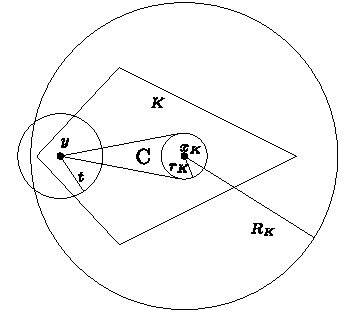
\includegraphics[width=0.7\linewidth,height=0.38\textheight,keepaspectratio]{dagpub-standalone-combined-2025-04-24-15-43-43-page-1.pdf2svg.pdf}\end{center}
 Figure 1: A property of fat convex sets. 
% END S2.F1
% BEGIN S2.SS0.SSS0.P0.SPx1
\par\medskip\noindent\textbf{Proof.}\par
Let $B(x_{K},r_{K})\subset K\subset B(x_{K},R_{K})$ with $R_{K}\leq\rho r_{K}$, and define $r_{K}^{\prime}=\min(r_{K},t)\geq t/\rho$ and $C=\operatorname{conv}(\{y\}\cup B(x_{K},r_{K}))\subset K$. $C$ contains all the points $u$ of $B(y,r_{K}^{\prime})$ such that $\angle(u-y,x_{K}-y)$ is at most some number depending only on $\rho$, so $C$ contains a constant fraction of $B(y,t)$. $\hfill\vartriangleleft$
\par
\par
\par
% END S2.SS0.SSS0.P0.SPx1
% BEGIN S2.SS0.SSS0.P0.SPx2
\par\medskip\noindent\textbf{Proof of Theorems 10 and 11.}\par
The proof is by induction on $k$ and $d$. Let $n_{i}=|\mathcal{F}_{i}|$. Let $\mathcal{H}$ be the $(k+2)$-uniform hypergraph with vertex set $\mathcal{F}=\cup\mathcal{F}_{i}$, where the edges are those colorful $(k+2)$-tuples which have a [spherical] $k$-transversal. Charge every hyperedge to its member $K$ with the smallest bounding radius $R_{K}$. In case of ties, charge arbitrarily to one of the members $K$ with smallest $R_{K}$.
\par
\par
Since in total there are $\alpha n_{1}\cdots n_{k+2}$ many charges, there is a color class $\mathcal{F}_{i}$ whose members are charged $\frac{\alpha}{k+2}n_{1}\cdots n_{k+2}$ times. Without loss of generality, we may assume that this color class is $\mathcal{F}_{k+2}$. Pick the set $K_{0}$ from $\mathcal{F}_{k+2}$ with the most charge. By averaging, $K_{0}$ was charged at least $\frac{\alpha}{k+2}n_{1}\cdots n_{k+1}$ times.
\par
\par
If $k=0$, then we have $\frac{\alpha}{2}n_{1}$ sets from $\mathcal{F}_{1}$ intersecting $K_{0}\in\mathcal{F}_{2}$. We have a point $y_{K}\in B(x_{K_{0}},R_{K_{0}})\cap K$ for all such $K\in\mathcal{F}_{1}$. Since $R_{K_{0}}\leq R_{K}$, the set $K$ contains a positive fraction of the ball $B(y_{K},R_{K_{0}})$ by Claim 12. Moreover, $B(y_{K},R_{K_{0}})$ occupies a positive fraction of $B(x_{K_{0}},2R_{K_{0}})$, so it follows that every $K$ contains a positive fraction of $B(x_{K_{0}},2R_{K_{0}})$. In this case, a constant fraction of the $\frac{\alpha}{2}n_{1}$ sets can be hit by a single point by the volumetric pigeonhole principle (where the constant depends only on the dimension and $\rho$).
\par
\par
If $k>0$, we can reduce finding a [spherical] $k$-transversal in $\mathbb{R}^{d}$ [in $\mathbb{S}^{d}$] to finding a spherical $(k-1)$-transversal in $\mathbb{S}^{d-1}$ as follows.
\par
\par
\par
% END S2.SS0.SSS0.P0.SPx2
% BEGIN S2.SS0.SSS0.P0.SPx3
\par\medskip\noindent\textbf{Euclidean case.}\par
If we are in the Euclidean space $\mathbb{R}^{d}$, we may assume that $B_{0}=B(x_{K_{0}},R_{K_{0}})$ is the unit ball centered at the origin. Let $K^{\prime}=K+B_{0}$ (where $+$ denotes the Minkowski sum) if $K\in\cup\mathcal{F}_{i}\setminus\{K_{0}\}$, and let $K_{0}^{\prime}$ be the degenerate ball containing only the origin. Denote the new families by $\mathcal{F}^{\prime}=\cup\mathcal{F}_{i}^{\prime}$.
\par
\par
\par\medskip\noindent\textbf{$\vartriangleright$ Claim 13.}\par
At least $\frac{\alpha}{k+2}n_{1}\cdots n_{k+1}$ of the colorful selections of $\mathcal{F}_{1}^{\prime},\ldots,\mathcal{F}_{k+1}^{\prime}$ have a $k$-dimensional linear subspace hitting them.
\par
\par
\par
\par
% END S2.SS0.SSS0.P0.SPx3
% BEGIN S2.SS0.SSS0.P0.SPx4
\par\medskip\noindent\textbf{Proof.}\par
The set $K_{0}$ was charged $\frac{\alpha}{k+2}n_{1}\cdots n_{k+1}$ times. Take $K_{1}\in\mathcal{F}_{1},\ldots,K_{k+1}\in\mathcal{F}_{k+1}$ such that $\{K_{0},K_{1},\ldots,K_{k+1}\}$ was charged to $K_{0}$ and translate their hitting $k$-flat to the origin. As the translation is by at most $R_{K_{0}}$, if any $K_{i}$ was hit by the original $k$-flat, then $K_{i}^{\prime}$ is hit by the translated (linear) $k$-flat. $\hfill\vartriangleleft$
\par
\par
Now, centrally project every set in $\mathcal{F}^{\prime}\setminus\{K_{0}^{\prime}\}$ to the surface of the unit sphere from the origin. (If a set contains the origin, its projection is the entire sphere.)
\par
\par
\par\medskip\noindent\textbf{$\vartriangleright$ Claim 14.}\par
A projection of a $\rho$-fat convex set is $\frac{\pi}{2}\rho$-fat.
\par
\par
\par
\par
% END S2.SS0.SSS0.P0.SPx4
% BEGIN S2.SS0.SSS0.P0.SPx5
\par\medskip\noindent\textbf{Proof.}\par
The projection of a ball $B(x,r)$ to the unit sphere centered at the origin is a cap of the unit sphere with radius $\sin^{-1}(r/t)$ if $x$ is at distance $t\geq r$ of the origin. Thus, the projection of a $\rho$-convex set $K$ is $\frac{\sin^{-1}(R_{K}/t)}{\sin^{-1}(r_{K}/t)}$-fat if $x_{K}$ is at distance $t>R_{K}$ from the origin. But $t\leq\sin^{-1}(t)\leq\frac{\pi}{2}t$, thus $\frac{\sin^{-1}(R_{K}/t)}{\sin^{-1}(r_{K}/t)}\leq\frac{\pi}{2}\frac{R_{k}}{r_{%
k}}=\frac{\pi}{2}\rho$ and the image of $K$ is $\frac{\pi}{2}\rho$-fat.
\par
\par
If $t\leq R_{K}$, then the projection of $B(x_{K},r_{K})$ is a cap with radius $\sin^{-1}(r_{K}/t)\geq\frac{r_{K}}{t}\geq\frac{1}{\rho}$. Either the projection of $K$ is contained in a cap of radius $\pi/2$ and contains a cap of radius $\frac{1}{\rho}$, or the image of $K$ is the complete unit sphere. In both cases the projection is $\frac{\pi}{2}\rho$-fat. $\hfill\vartriangleleft$ Denote the obtained family of $\rho^{\prime}=\frac{\pi}{2}\rho$-fat spherically convex sets by $\mathcal{F}^{*}$. As $\frac{\alpha}{k+2}n_{1}\cdots n_{k+1}$ of the colorful selections of $\mathcal{F}_{1}^{\prime},\ldots,\mathcal{F}_{k+1}^{\prime}$ have a $k$-dimensional linear subspace hitting them by Claim 13, we have that $\frac{\alpha}{k+2}n_{1}\cdots n_{k+1}$ of the colorful selections of $\mathcal{F}_{1}^{*},\ldots,\mathcal{F}_{k+1}^{*}$ have a great $(k-1)$-sphere intersecting them. The assumptions of the spherical colorful fractional Helly Theorem 11 on $\mathbb{S}^{d-1}$ with great $(k-1)$-spheres are satisfied, thus we have an $i\in[k+1]$ and a subfamily $\mathcal{G}^{*}\subset\mathcal{F}_{i}^{*}$ of size at least $\beta^{*}|\mathcal{F}_{i}^{*}|$ which can be hit by a great $(k-1)$-sphere, where $\beta^{*}$ is the value we obtain from Theorem 11 with parameters $d-1,k-1$ and $\frac{\alpha}{k+2}$. This means that the corresponding family of preimages $\mathcal{G}^{\prime}=\{K^{\prime}\in\mathcal{F}^{\prime}:\operatorname{proj}_{%
\mathbb{S}^{d-1}}K^{\prime}\in\mathcal{G}^{*}\}$ can be hit by a $k$-dimensional linear subspace $F$. Let $\mathcal{G}=\{K\in\mathcal{F}:K^{\prime}\in\mathcal{G}^{\prime}\}$. If we project $K_{0}$ and every set $K\in\mathcal{G}$ to the orthogonal complement $F^{\perp}$ of $F$, every projected set $\operatorname{proj}_{F^{\perp}}K$ will intersect the set $\operatorname{proj}_{F^{\perp}}K_{0}$.
\par
\par
Since for all $K$ there exists a $y_{K}\in B(0,1)\cap\operatorname{proj}_{F^{\perp}}K$, and $\operatorname{proj}_{F^{\perp}}K$ contains a ball of $F^{\perp}$ of radius $\rho$, we know that $K$ occupies a constant fraction of $B(y_{K},1)\cap F^{\perp}\subset B(0,2)\cap F^{\perp}$ by Claim 12 and thus a positive fraction of $B(0,2)\cap F^{\perp}$. By the pigeonhole principle we can find a point $x\in F^{\perp}$ in the intersection of a constant fraction of the projections $\{\operatorname{proj}_{F^{\perp}}K:K\in\mathcal{G}^{\prime}\}$. $F+x$ (the translation of $F$ by $x$) is a $k$-flat intersecting a constant fraction of the fat convex sets in $\mathcal{G}^{\prime}$.
\par
\par
\par
% END S2.SS0.SSS0.P0.SPx5
% BEGIN S2.SS0.SSS0.P0.SPx6
\par\medskip\noindent\textbf{Spherical case.}\par
For this case, we need some claims about the geometry of spherical caps and great $k$-spheres which are described in Section 3, but otherwise the main argument is the same as in the Euclidean case. First, we deal with the case where there are many large sets in $\cup_{i}\mathcal{F}_{i}$. Note that we may assume that all the $n_{i}$s are large enough, otherwise a $\beta$-fraction of a color class will consists of a single set $K$ (if $\beta$ is chosen to be small enough). Let $c<\alpha/(k+2)$ be a small constant. If there is an $\mathcal{F}_{i}$ such that for at least $cn_{i}$ of the sets $K\in\mathcal{F}_{i}$ we have $R_{K}>\pi/8$, then a constant fraction of them can be hit with a single point by the volumetric pigeonhole principle, as all of them contain caps with radius at least $\rho\pi/8$. This constant fraction depends only on $d$ and $\rho$. If we do not have this many large sets in any of the $\mathcal{F}_{i}$, we can simply delete the large ones, as this way we loose at most $c(k+2)n_{1}\ldots n_{k+2}$ out of the original $\alpha n_{1}\ldots n_{k+2}$ colorful $(k+2)$-tuples with a spherical $k$-transversal. Thus, we can have families of size at least $(1-c)n_{i}$ with at least an $(\alpha-c(k+2))n_{1}\ldots n_{k+2}$ colorful $(k+2)$-tuples having a spherical $k$-transversal and no set $K$ in the families with $R_{K}>\pi/8$.
\par
\par
Let $K_{0}$ be the most charged set as defined above, let $\varepsilon=R_{K_{0}}$ and $B_{0}=B(x_{K_{0}},\varepsilon)$. For a set $K\subset\mathbb{S}^{d}$, its $\varepsilon$-neighborhood is $K^{\varepsilon}=\{u\in\mathbb{S}^{d}:\exists v\in K\text{ with }\angle(u,v)%
\leq\varepsilon\}$, and $\operatorname{conv}(K)$ is the intersection of all the spherically convex sets containing $K$. If $K$ is a $\rho$-fat convex set, then $\operatorname{conv}(K^{\varepsilon})$ is a $\rho$-fat convex set by Claim 15. For every $K\in\cup\mathcal{F}_{i}\setminus\{K_{0}\}$, let $K^{\prime}=\operatorname{conv}(K^{\varepsilon})$ and let $K_{0}^{\prime}=\{x_{K_{0}}\}$. Denote the new families of spherically convex $\rho$-fat sets by $\mathcal{F}^{\prime}=\cup\mathcal{F}_{i}^{\prime}$. By Claim 16, if some sets in $\mathcal{F}$ can be hit by a great $k$-sphere, then the corresponding sets in $\mathcal{F}^{\prime}$ can be hit by a great $k$-sphere as well. Now let $\mathcal{F}^{*}=\operatorname{proj}_{B_{0}}\mathcal{F}^{\prime}$, where $\operatorname{proj}_{B_{0}}$ denotes the projection into the boundary $\partial B_{0}$. By Claim 19, $\mathcal{F}^{*}$ is a family of spherically convex $\rho^{\prime}=\frac{\pi^{3}}{4}\rho^{2}$-fat sets of the $(d-1)$-dimensional sphere $\partial B_{0}$. Without loss of generality, assume that $K_{0}\in\mathcal{F}_{k+2}$. As $K_{0}$ is the most charged set, at least $\frac{\alpha}{k+2}$-fraction of the colorful selections of $\mathcal{F}_{1}^{\prime},\ldots,\mathcal{F}_{k+1}^{\prime}$ have a spherical $k$-transversal containing $x_{0}$. These great $k$-spheres of $\mathbb{S}^{d}$ become great $(k-1)$-spheres of $\partial B_{0}$ after the projection. Thus, at least $\frac{\alpha}{k+2}$-fraction of the colorful selections of $\mathcal{F}_{1}^{*},\ldots,\mathcal{F}_{k+1}^{*}$ have a $(k-1)$-transversal. The assumptions of the spherical colorful fractional Helly Theorem 11 on $\partial B_{0}$ with spherical $(k-1)$-transversals are satisfied, thus we have an $i$ and a subfamily $\mathcal{G}^{*}\subset\mathcal{F}_{i}^{*}$ of size at least $\beta^{*}|\mathcal{F}_{i}^{*}|$ which has a spherical $(k-1)$-transversal. This means that the corresponding family of preimage sets $\mathcal{G}^{\prime}$ has a spherical $k$-transversal. By Claim 20, a large subfamily of $\mathcal{G}$ has a spherical $k$-transversal as well. $\hfill\blacktriangleleft$
\par
\par
\par
% END S2.SS0.SSS0.P0.SPx6
% END S2
% BEGIN S3
\par\medskip\noindent\textbf{3 Caps and projections on the sphere}\par
% BEGIN S3.p1
In this section, we prove the claims about spherical sets that were used in the proof of Theorem 11. All the arguments are fairly straight-forward modifications of the simple proofs used in the Euclidean case, but more tedious calculations are required.
\par
\par
% END S3.p1
% BEGIN S3.p2
Recall that $B(v,\varepsilon)$ is the spherical cap centered at $v$ with angle $\varepsilon$, and a great $k$-sphere of $\mathbb{S}^{d}$ is the intersection of $\mathbb{S}^{d}$ with a $(k+1)$-dimensional linear subspace of $\mathbb{R}^{d+1}$ [4]. A great $1$-sphere is called a great circle.
\par
\par
% END S3.p2
% BEGIN S3.p3
For $u\in\mathbb{S}^{d}\setminus\{v,-v\}$, let $\operatorname{rot}(u,v)$ be the rotation $r$ with $r(u)=v$ which is constant on $\operatorname{span}(\{u,v\})^{\perp}$, so we rotate with the $uov$ angle $\angle(u,v)$ around the center $o$, keeping $\operatorname{span}(\{u,v\})^{\perp}$ fixed. If $u\notin\{v,-v\}$, the projection of $u\in\mathbb{S}^{d}$ onto the boundary $\partial B(v,\varepsilon)$ of the cap $B(v,\varepsilon)$ is the intersection of $\partial B(v,\varepsilon)$ with the halfplane embedded in $\mathbb{R}^{d+1}$ containing $o$ and $v$ on its boundary, and $u$ in its interior. In other words, if $u\not\in B(v,\varepsilon)$, then the projection is the point of $\partial B(v,\varepsilon)$ that is hit when we rotate $u$ to $v$. It is denoted by $\operatorname{proj}_{B}(u)$, or simply $\operatorname{proj}(u)$ if $B$ is clear from the context. For any set $X$ and cap $B=B(v,\varepsilon)$, let $\operatorname{proj}_{B}X=\{\operatorname{proj}_{B}(u):u\in X\}$ if $X\cap\{v,-v\}=\emptyset$, and let $\operatorname{proj}_{B}X=B$ if $X\cap\{v,-v\}\neq\emptyset$.
\par
\par
% END S3.p3
% BEGIN Thmtheorem15
\par\medskip\noindent\textbf{$\vartriangleright$ Claim 15.}\par
If $K\subseteq\mathbb{S}^{d}$ is $\rho$-fat, then $\operatorname{conv}(K^{\varepsilon})$ is $\rho$-fat as well.
\par
\par
\par
% END Thmtheorem15
% BEGIN S3.SS0.SSS0.P0.SPx1
\par\medskip\noindent\textbf{Proof.}\par
If $\operatorname{conv}(K^{\varepsilon})=\mathbb{S}^{d}$, then it is $\rho$-fat with $\rho=1$. Otherwise, as $B(x_{K},r_{K}+\varepsilon)\subseteq\operatorname{conv}(K^{\varepsilon})%
\subseteq B(x_{K},R_{K}+\varepsilon)$, the $\rho$-fatness of $K^{\varepsilon}$ follows from $\frac{R_{K}+\varepsilon}{r_{K}+\varepsilon}\leq\frac{R_{K}}{r_{K}}\leq\rho$. $\hfill\vartriangleleft$
\par
\par
\par\medskip\noindent\textbf{$\vartriangleright$ Claim 16.}\par
If the spherical sets $K_{1},\ldots,K_{n}\subset\mathbb{S}^{d}$ can be pierced with a great $k$-sphere, and $K_{1}\subset B(v,\varepsilon)$, then $B(v,0),K_{2}^{\varepsilon},\ldots,K_{n}^{\varepsilon}$ can also be pierced with a great $k$-sphere.
\par
\par
\par
\par
% END S3.SS0.SSS0.P0.SPx1
% BEGIN S3.SS0.SSS0.P0.SPx2
\par\medskip\noindent\textbf{Proof.}\par
Take a great $k$-sphere $F$ intersecting all of $K_{1},\ldots,K_{n}\subset\mathbb{S}^{d}$, let $v^{\prime}=\operatorname{proj}_{F}(v)$ and $\operatorname{rot}=\operatorname{rot}(v^{\prime},v)$. For any point $u\in\mathbb{S}^{d}$, the spherical distance between $u$ and $\operatorname{rot}(u)$ is at most $\varepsilon$. Hence, if $u\in K_{i}\cap F$, then $\operatorname{rot}(u)\in K_{i}^{\varepsilon}\cap\operatorname{rot}(F)$, thus the great $k$-sphere $\operatorname{rot}(F)$ intersects all of $B(v,0),K_{2}^{\varepsilon},\ldots,K_{n}^{\varepsilon}$. $\hfill\vartriangleleft$
\par
\par
We want to show that during a gnomonic projection the distance of two points close to the center of the projected image cannot be distorted too much. This is probably a well-known statement, but we could not find it anywhere, so we include the simple calculation below. If we embed $\mathbb{S}^{d}$ into $\mathbb{R}^{d+1}$ as the unit sphere, the spherical distance of $x$ and $y$ becomes $\angle(x,y)$, while their Euclidean distance is $|x-y|$.
\par
\par
\par\medskip\noindent\textbf{$\vartriangleright$ Claim 17.}\par
Embed $\mathbb{S}^{d}$ into $\mathbb{R}^{d+1}$ as the unit sphere. If $u,v\in B(w,\pi/4)\subset\mathbb{S}^{d}$ and $p$ is the central projection from the origin to the supporting hyperplane of $\mathbb{S}^{d}$ at $w$, then we have $\angle(u,v)\leq|p(u)-p(v)|\leq 2\angle(u,v)$.
\par
\par
\par
\par
% END S3.SS0.SSS0.P0.SPx2
% BEGIN S3.SS0.SSS0.P0.SPx3
\par\medskip\noindent\textbf{Proof.}\par
As $u,v,w$ are contained in a $2$-dimensional subsphere, it is enough to show the claim for $d=2$. First we calculate the distortion of length if $u$ and $w$ have the same latitude of longitude.
\par
\par
Case 1: $u,v,w$ are on the same great circle. As we have $|p(u)-w|=\tan(\angle(u,w))$ and $1\leq\tan^{\prime}(\varphi)\leq 2$ if $\varphi\in(0,\pi/4)$, we have $\angle(u,v)\leq|u-v|\leq 2\angle(u,v)$.
\par
\par
Case 2: $\angle(u,w)=\angle(v,w)=\varphi$. In this case $p$ acts on them as a homothety with ratio $1/\cos(\varphi)$, which is between $1$ and $\sqrt{2}$ if $\varphi\in(0,\pi/4)$.
\par
\par
We can argue that these are the extreme cases and the distortion of length is always between $1$ and $2$. We show that for close enough points the distortion of distance is between $1$ and $2$. But then the global distortion has to be in the same interval.
\par
\par
For every $u\in B(w,\pi/4)$ the points of $\mathbb{S}^{d}$ with a small enough given distance from $u$ form a circle inside $B(w,\pi/4)$. Its image under $p$ is an ellipse. Due to symmetry the axes of the ellipse correspond to point pairs with the same latitude or longitude. We have seen in Cases 1 and 2 that the ratios of the lengths of the axes and the radius of the circle are between $1$ and $2$. But then for every point $v$ in the circle we have $\angle(u,v)\leq|p(u)-p(v)|\leq 2\angle(u,v)$. $\hfill\vartriangleleft$
\par
\par
\par\medskip\noindent\textbf{$\vartriangleright$ Claim 18.}\par
If $K\subseteq B(w,\pi/8)\subset\mathbb{S}^{d}$ is convex and $\varepsilon\leq\pi/8$, then $\operatorname{conv}(K^{\varepsilon})\subset K^{2\varepsilon}$.
\par
\par
\par
\par
% END S3.SS0.SSS0.P0.SPx3
% BEGIN S3.SS0.SSS0.P0.SPx4
\par\medskip\noindent\textbf{Proof.}\par
If $u\in\operatorname{conv}(K^{\varepsilon})$, then there are $u^{\prime},u^{\prime\prime}\in K^{\varepsilon}$ such that $u\in\operatorname{conv}(\{u^{\prime},u^{\prime\prime}\})$. Let $v^{\prime},v^{\prime\prime}\in K$ be such that $\angle(u^{\prime},v^{\prime}),\angle(u^{\prime\prime},v^{\prime\prime})\leq\varepsilon$. Let $p$ be the central projection of $B(w,\pi/4)$ from the origin to the supporting hyperplane of $\mathbb{S}^{d}$ at $w$. As $u^{\prime},u^{\prime\prime},v^{\prime},v^{\prime\prime}\in B(w,\pi/4)$, we have $|p(u^{\prime})-p(v^{\prime})|,|p(u^{\prime\prime})-p(v^{\prime\prime})|\leq 2\varepsilon$ by Claim 18. As the projections of $\operatorname{conv}(\{u^{\prime},u^{\prime\prime}\})$ and $\operatorname{conv}(\{v^{\prime},v^{\prime\prime}\})$ are segments of a Euclidean space whose endpoints have distance at most $2\varepsilon$, there is a point $v\in\operatorname{conv}(\{v^{\prime},v^{\prime\prime}\})$ such that $|p(v)-p(u)|\leq 2\varepsilon$. We have $\angle(u,v)\leq 2\varepsilon$ by Claim 18. As $v\in K$, this proves $u\in K^{2\varepsilon}$. $\hfill\vartriangleleft$
\par
\par
\par\medskip\noindent\textbf{$\vartriangleright$ Claim 19.}\par
Let $B=B(v,\varepsilon)$ be a cap, and $K$ be a $\rho$-fat convex set of $\mathbb{S}^{d}$. The projection $\operatorname{proj}_{B}K$ is a $\frac{\pi^{3}}{4}\rho^{2}$-fat convex set of the $(d-1)$-dimensional sphere $\partial B$.
\par
\par
\par
\par
% END S3.SS0.SSS0.P0.SPx4
% BEGIN S3.SS0.SSS0.P0.SPx5
\par\medskip\noindent\textbf{Proof.}\par
If $\operatorname{proj}_{B}K=B$, then it is convex by definition. Otherwise, as $\operatorname{proj}_{B}$ maps (shorter) great circle arcs to (shorter) great circle arcs or points, the projection is convex. Let $\rho^{\prime}=\frac{\pi^{3}}{4}\rho^{2}$. To show $\rho^{\prime}$-fatness, we need to examine how the radius of $B(x_{K},r_{K})\subset K$ and $B(x_{K},R_{K})\supset K$ change after the projection.
\par
\par
Assume that $B(x,r)$ is any cap of $\mathbb{S}^{d}$ and $v\not\in B(x,r)$. Embed $\mathbb{S}^{d}$ in $\mathbb{R}^{d+1}$ as the unit sphere and look at the simplex spanned by $\underline{0},x,v$ and $b$ where $b\in\partial B(x,r)$. The radius $\varphi$ of $\operatorname{proj}_{B(v,\varepsilon)}B(x,r)$ will be $\max_{b}\angle(b-v,x-v)$.
\par
\par
As $\frac{\sin\angle(b-v,x-v)}{|x-b|}=\frac{\sin\angle(x-b,v-b)}{|x-v|}$ by the law of sines, $\angle(b-v,x-v)$ is maximal if $\angle(x-b,v-b)=\pi/2$. Fix such a $b$. We have $\sin\varphi=\frac{|x-b|}{|x-v|}$.
\par
\par
Let $\angle(v,x)=t$. As $|x|=|v|=|b|=1$, we have $|x-v|=2-2\cos t$ and $|x-b|=2-2\cos r$ by the law of cosines. As $1-\cos t=\sin^{2}(t/2)$ and $\sin t\leq t$, we have $\varphi\geq\sin\varphi=\frac{|x-b|}{|x-v|}=\frac{\sin^{2}(r/2)}{\sin^{2}(t/2)}$. If $\varphi\leq\pi/2$, then we also have $\varphi\leq\frac{\pi}{2}\sin\varphi=\frac{\pi}{2}\frac{\sin^{2}(r/2)}{\sin^{2}%
(t/2)}$.
\par
\par
Now returning to the proof, for simplicity we will write $\operatorname{proj}$ for $\operatorname{proj}_{B}$. Let $\varphi_{r}$ and $\varphi_{R}$ be such that $\operatorname{proj}B(x_{K},r_{K})=B(\operatorname{proj}x_{K},\varphi_{r})$ and $\operatorname{proj}B(x_{K},R_{K})=B(\operatorname{proj}x_{K},\varphi_{R})$.
\par
\par
If $\varphi_{R}\geq\pi/2$, then $R\geq t$. In this case we have either $\varphi_{r}\geq\pi/2$ or $\varphi_{r}\geq\sin\varphi_{r}=\frac{\sin^{2}(r/2)}{\sin^{2}(t/2)}\geq\frac{4}%
{\pi^{2}}\frac{r^{2}}{t^{2}}\geq\frac{4}{\pi^{2}}\frac{r^{2}}{t^{2}}\geq\frac{%
4}{\pi^{2}\rho^{2}}$ and so $\varphi_{R}\leq\pi\leq\frac{\pi^{3}}{4}\rho^{2}\varphi_{r}$.
\par
\par
Otherwise $\varphi_{R}<\varphi/2$ and we have $\frac{\varphi_{R}}{\varphi_{r}}\leq\frac{\pi}{2}\frac{\sin\varphi_{R}}{\sin%
\varphi_{r}}=\frac{\pi}{2}\frac{\sin^{2}(R/2)}{\sin^{2}(r/2)}\leq\frac{\pi^{3}%
}{8}\frac{R^{2}}{r^{2}}\leq\frac{\pi^{3}}{8}\rho^{2}$. As $\operatorname{proj}B(x_{K},r_{K})\subset\operatorname{proj}K\subset%
\operatorname{proj}B(x_{K},R_{K})$, in this case $K$ is $\frac{\pi^{3}}{8}\rho^{2}$-fat. $\hfill\vartriangleleft$
\par
\par
\par\medskip\noindent\textbf{$\vartriangleright$ Claim 20.}\par
For every $d$, $\rho$ and $k$ there exists a constant $c>0$ such that the following holds for every $\varepsilon>0$. Let $K_{2},\ldots,K_{n}$ be $\rho$-fat convex sets of $\mathbb{S}^{d}$ with $\varepsilon\leq R_{K_{i}}$ for all $i\in\{2,\ldots,n\}$. If $\operatorname{conv}(K_{2}^{\varepsilon}),\ldots,\operatorname{conv}(K_{n}^{%
\varepsilon})$ can be hit with a great $k$-sphere, then $cn$ sets from $K_{2},\ldots,K_{n}$ can be hit with a great $k$-sphere as well.
\par
\par
\par
\par
% END S3.SS0.SSS0.P0.SPx5
% BEGIN S3.SS0.SSS0.P0.SPx6
\par\medskip\noindent\textbf{Proof.}\par
If $R_{K_{i}}\geq\pi/8$ for at least half of the sets, then, as those sets all contain caps of radius at least $\pi/(8\rho)$, a constant fraction of them can be hit even with a single point by the volumetric pigeonhole principle. Otherwise delete all the sets $K_{i}$ with $R_{K_{i}}\geq\pi/8$ and at least half of the sets remain. Let the family of the remaining at least $n/2$ sets be $\mathcal{H}$.
\par
\par
Let $F$ be the great $k$-sphere hitting all the sets of $\{\operatorname{conv}(K^{\varepsilon}):K\in\mathcal{H}\}$. In this case, all $K\in\mathcal{H}$ are at distance at most $2\varepsilon$ from $F$ by Claim 18.
\par
\par
If $k=0$, let $F=\{\pm v\}$. For all $K\in\mathcal{H}$ there exists a $y_{K}\in K$ which is at distance at most $2\varepsilon$ from one of the two antipodal points of $F$. As $K$ occupies a constant fraction of $B(y_{K},\varepsilon)$ by Claim 12 and $B(y_{K},\varepsilon)$ contains a constant fraction of $B(v,2\varepsilon)\cup B(-v,2\varepsilon)$, the volumetric pigeonhole principle yields a point intersecting $cn$ of the sets of $\mathcal{H}$.
\par
\par
We can reduce the $k>0$ case to the $k=0$ case with a suitable projection. For a $K\in\mathcal{H}$, let $f(K)$ be a closest point of $F$ to $K$. Let $\delta=\delta(d,k)>0$ be a small enough number, and let $N$ be a metric $\delta$-net of $F$ (its size depends only on $k$ and $d$). By the pigeonhole principle, there exists a point $u\in N$ and a subfamily $\mathcal{H}^{\prime}\subset\mathcal{H}$ with $|\mathcal{H}^{\prime}|\geq c^{\prime}|\mathcal{H}|$ such that for all $K\in\mathcal{H}^{\prime}$, the point $f(K)$ has distance at most $\delta$ from $u$.
\par
\par
Embed $\mathbb{S}^{d}$ into $\mathbb{R}^{d+1}$ as the unit sphere and let $V$ be the $(k+1)$-dimensional linear subspace of $\mathbb{R}^{d+1}$ with $V\cap\mathbb{S}^{d}=F$. Let $u,u_{1},\ldots,u_{k}$ be an orthonormal basis of $V$. Let $B_{i}=B(u_{i},\pi/2)$ be the halfsphere centered at $u_{i}$, let $\operatorname{proj}_{i}=\operatorname{proj}_{B_{i}}$ be the projection from $\mathbb{S}^{d}$ to $\partial B_{i}$ as defined above, and let $\operatorname{proj}_{F,u}=\operatorname{proj}_{1}\circ\operatorname{proj}_{2}%
\circ\ldots\circ\operatorname{proj}_{k}$. The repeated application of Claim 19 gives us that if $K\subset\mathbb{S}^{d}$ is a $\rho$-fat convex set, then $\operatorname{proj}_{F_{u}}K$ is a $\rho^{\prime}=c^{k}\rho^{2k}$-fat convex set where $c\geq 1$ is a universal constant.
\par
\par
Apply $\operatorname{proj}_{F,u}$ to $F$ and the sets of $\mathcal{H}^{\prime}$ to get projections in the great $(d-k)$-sphere $\partial B_{2}\cap\ldots\cap\partial B_{k}$. This way $F$ becomes a pair of antipodal points $\{\pm u\}$, the projections of members of $\mathcal{H}^{\prime}$ are $\rho^{\prime}$-fat, and if $\delta(d,k)$ is sufficiently small, they are at distance at most $3\varepsilon$ from $u$. By the $k=0$ case we can find a point intersecting a constant fraction of the sets in $\{\operatorname{proj}_{F,u}K:K\in\mathcal{H}^{\prime}\}$. The preimage of this point under $\operatorname{proj}_{F,u}$ is part of a great $k$-sphere of $\mathbb{S}^{d}$, and hits a constant fraction of $\mathcal{H}^{\prime}$, thus a constant fraction of $\mathcal{H}$ and of $\{K_{2},\ldots,K_{n}\}$. $\hfill\vartriangleleft$
\par
\par
\par
% END S3.SS0.SSS0.P0.SPx6
% END S3

% BEGIN S4
\par\medskip\noindent\textbf{4 $(p,k+2)$-theorems}\par
% BEGIN S4.p1
The specific $\rho=1$ case of the fractional Helly results of Section 2 implies $(p,q)$-type results for $k$-flats intersecting balls. In this section we summarize arguments showing that Theorem 10 implies Theorem 8. The following colorful generalization can also be proved with a variant of this method. To keep the presentation simple, we only describe the arguments in a non-colorful setting. The interested reader can find a version of the colorful arguments in [5].
\par
\par
% END S4.p1
% BEGIN Thmtheorem21
\par\medskip\noindent\textbf{Theorem 21.}\par
For every three positive integers $d$, $k<d$ and $p\geq k+2$ there exists a $C$ such that the following holds. If $\mathcal{F}_{1},\ldots,\mathcal{F}_{p}$ are families of closed balls in $\mathbb{R}^{d}$ such that for every $B_{1}\in\mathcal{F}_{1},\ldots,B_{p}\in\mathcal{F}_{p}$ there are $k+2$ balls that can be hit by a single $k$-flat, then there exist an $i\in[p]$ and at most $C$ $k$-flats hitting all balls of $\mathcal{F}_{i}$.
\par
\par
\par
% END Thmtheorem21
% BEGIN S4.p2
By the same method, the following is a corollary of Theorem 11.
\par
\par
% END S4.p2
% BEGIN Thmtheorem22
\par\medskip\noindent\textbf{Theorem 22.}\par
For every three positive integers $d$, $k<d$ and $p\geq k+2$ there exists a $C$ such that the following holds. If $\mathcal{F}_{1},\ldots,\mathcal{F}_{p}$ are finite families of closed caps in $\mathbb{S}^{d}$ such that for every $B_{1}\in\mathcal{F}_{1},\ldots,B_{p}\in\mathcal{F}_{p}$ there are $k+2$ caps that can be hit by a great $k$-sphere, then there exist an $i\in[p]$ and at most $C$ great $k$-spheres hitting all caps of $\mathcal{F}_{i}$.
\par
\par
\par
% END Thmtheorem22
% BEGIN S4.p3
Note that the case where the families of balls (caps) can be infinite follows from the finite case by a standard compactness argument. The proofs of the finite versions are simple applications of the Alon-Kleitman method established in [3], later described in a more general setting in [2], and adapted to colorful variants in [5]. The abstract (purely combinatorial) proof described in [2] has two main steps. To state them, we phrase the fractional Helly and $(p,q)$-theorems in an abstract, purely combinatorial language as follows.
\par
\par
% END S4.p3
% BEGIN S4.p4
Let $\mathcal{H}$ be a set system over the base set $V$. For an integer $q$ and a function $\beta\colon(0,1]\to(0,1]$, the set system $\mathcal{H}$ satisfies the fractional Helly property FH($q,\beta$) if the following holds. For every $\alpha>0$ and every finite family $\mathcal{G}\subset\mathcal{H}$, if $\alpha\binom{|\mathcal{G}|}{q}$ of the $q$-tuples of $\mathcal{G}$ has a nonempty intersection, then there exists a subfamily $\mathcal{G}^{\prime}\subset\mathcal{G}$ of size $\beta(\alpha)|\mathcal{G}|$ such that all the members of $\mathcal{G}^{\prime}$ have an element of $V$ in common. The fractional Helly theorem of Katchalski and Liu (Theorem 1) states that if $V=\mathbb{R}^{d}$, and $\mathcal{H}$ consists of all the convex sets, then there exists $\beta$ such that $\mathcal{H}$ satisfies FH($d+1,\beta$). Our Theorem 5 states that if $V=\{k\text{-flats of }\mathbb{R}^{d}\}$ and $\mathcal{H}$ consists of families of $k$-flats intersecting a common $\rho$-fat convex set, then $\mathcal{H}$ satisfies FH($k+2,\beta$) with some $\beta$.
\par
\par
% END S4.p4
% BEGIN S4.p5
A set system $\mathcal{H}$ satisfies the $(p,q)$-condition if among any $p$ members of $\mathcal{H}$, some $q$ intersect. Note that for $p\geq q\geq r$, the $(p,q)$-condition implies the $(p,r)$-condition. The transversal number $\tau(\mathcal{H})$ denotes the minimum size of a set $T\subset V$ with $T\cap H\neq\emptyset$ for all $H\in\mathcal{H}$. The fractional transversal number $\tau^{*}(\mathcal{H})$ is the minimum $\sum_{v\in V}t(v)$ over functions $t\colon V\to[0,1]$ with $\sum_{v\in H}t(v)\geq 1$ for all $H\in\mathcal{H}$. Alon, Kalai, Matoušek and Meshulam proved the following two theorems.
\par
\par
% END S4.p5
% BEGIN Thmtheorem23
\par\medskip\noindent\textbf{Theorem 23 (Theorem 8 in Alon, Kalai, Matoušek and Meshulam [2]).}\par
If $\mathcal{H}$ satisfies FH($q,\beta$) and the $(p,q)$-condition with some $p\geq q$, then $\tau^{*}(\mathcal{H})\leq O_{p,q,\beta}(1)$.
\par
\par
\par
% END Thmtheorem23
% BEGIN S4.p6
Let $\mathcal{H}^{\cap}$ be the family of all sets that are the intersections of some members of $\mathcal{H}$.
\par
\par
% END S4.p6
% BEGIN Thmtheorem24
\par\medskip\noindent\textbf{Theorem 24 (Theorem 9 in Alon, Kalai, Matoušek and Meshulam [2]).}\par
For every $q$ and $\beta$ there exists a function $f_{q,\beta}$ such that if $\mathcal{H}^{\cap}$ satisfies FH($q,\beta$), then $\tau(\mathcal{H})\leq f_{q,\beta}(\tau^{*}(\mathcal{H}))$.
\par
\par
\par
% END Thmtheorem24
% BEGIN S4.p7
Note that if $\mathcal{H}^{\cap}$ satisfies $F(q,\beta)$ and $\mathcal{H}$ satisfies the $(p,q)$ condition, then its transversal number is bounded by a function of $p,q$ and $\beta$ as a consequence of the above two theorems. As the family of convex sets of $\mathbb{R}^{d}$ is closed under intersection, and satisfies $FH(d+1,\beta)$, this provides an alternative proof of Theorem 6 of Alon and Kleitman. But the same reasoning is usually not applicable to questions about $k$-transversals with $k>0$, as the corresponding $\mathcal{H}^{\cap}\neq\mathcal{H}$ is hard to analyze, for example, for balls the intersections are no longer fat. However, in this special case, another proof method works.
\par
\par
% END S4.p7
% BEGIN S4.p8
If we restrict the question to $k$-transversals of balls [caps], as in Theorem 21 [Theorem 22], then we can bound $\tau$ as a function of $\tau^{*}$ and thus prove our $(p,k+2)$-theorems. The bound on $\tau$ follows from a classical result of Haussler and Welzl [9] . The VC-dimension of $\mathcal{H}$ is the supremum of the sizes of subsets $S\subseteq V$ such that for every $X\subseteq S$ there is an $H\in\mathcal{H}$ satisfying $H\cap S=X$.
\par
\par
% END S4.p8
% BEGIN Thmtheorem25
\par\medskip\noindent\textbf{Theorem 25 (Haussler and Welzl [9]).}\par
For every $d$ there exists a function $f_{d}$ such that if $\mathcal{H}$ has VC-dimension at most $d$, then $\tau(\mathcal{H})\leq f_{d}(\tau^{*}(\mathcal{H}))$.
\par
\par
\par
% END Thmtheorem25
% BEGIN S4.p9
The VC-dimension of $k$-flats intersecting balls [caps] is bounded by the Milnor-Thom theorem on sign patterns of polynomials [18, 20], because a family of $k$-flats intersecting a given ball [cap] can be described by a bounded number of polynomial inequalities of bounded degree.
\par
\par
% END S4.p9
% BEGIN S4.p10
As for $k$-flats intersecting $\rho$-fat convex sets neither Theorem 24, nor Theorem 25 is applicable, the missing ingredient is proving a $(p,q)$-theorem for $k$-flats intersecting $\rho$-fat convex sets.
\par
\par
% END S4.p10
% BEGIN Thmtheorem26
\par\medskip\noindent\textbf{Conjecture 26.}\par
There is a function $f$ such that if $\mathcal{H}$ consists of families of $k$-flats intersecting members of a family of $\rho$-fat convex sets in $\mathbb{R}^{d}$, then $\tau(\mathcal{H})\leq f(\tau^{*}(\mathcal{H}))$.
\par
\par
\par
% END Thmtheorem26
% END S4
% BEGIN bib
\par\medskip\noindent\textbf{References}\par
\begin{enumerate}
\item[]  [1]  Noga Alon and Gil Kalai.  Bounding the piercing number.  Discrete \& Computational Geometry, 13:245–256, 1995.  doi:10.1007/BF02574042.  
\item[]  [2]  Noga Alon, Gil Kalai, Jiří Matoušek, and Roy Meshulam.  Transversal numbers for hypergraphs arising in geometry.  Advances in Applied Mathematics, 29(1):79–101, 2002.  doi:10.1016/S0196-8858(02)00003-9.  
\item[]  [3]  Noga Alon and Daniel J Kleitman.  Piercing convex sets and the Hadwiger-Debrunner $(p,q)$-problem.  Advances in Mathematics, 96(1):103–112, 1992.  
\item[]  [4]  Boris Aronov, Jacob E Goodman, and Richard Pollack.  A Helly-type theorem for higher-dimensional transversals.  Computational Geometry, 21(3):177–183, 2002.  doi:10.1016/S0925-7721(01)00025-6.  
\item[]  [5]  Imre Bárány, Ferenc Fodor, Luis Montejano, Deborah Oliveros, and Attila Pór.  Colourful and fractional $(p,q)$-theorems.  Discrete \& Computational Geometry, 51(3):628–642, 2014.  doi:10.1007/S00454-013-9559-0.  
\item[]  [6]  Arijit Ghosh and Soumi Nandi.  Heterochromatic higher order transversals for convex sets.  arXiv preprint arXiv:2212.14091 version 1, 2022.  doi:10.48550/arXiv.2212.14091.  
\item[]  [7]  Jacob E Goodman, Richard Pollack, and Rephael Wenger.  Geometric transversal theory.  In New trends in discrete and computational geometry, pages 163–198. Springer, 1993.  
\item[]  [8]  Hugo Hadwiger and Hans Debrunner.  Über eine Variante zum Hellyschen Satz.  Archiv der Mathematik, 8:309–313, 1957.  doi:10.1007/BF01898794.  
\item[]  [9]  David Haussler and Emo Welzl.  Epsilon-nets and simplex range queries.  In Proceedings of the second annual symposium on Computational geometry, pages 61–71, 1986.  doi:10.1145/10515.10522.  
\item[]  [10]  Eduard Helly.  Über Mengen konvexer Körper mit gemeinschaftlichen Punkten.  Jahresbericht der Deutschen Mathematiker-Vereinigung, 32:175–176, 1923.  
\item[]  [11]  Andreas Holmsen and Jiří Matoušek.  No Helly theorem for stabbing translates by lines in $\mathbb{R}^{3}$.  Discrete \& Computational Geometry, 31(3):405–410, 2004.  doi:10.1007/s00454-003-0796-5.  
\item[]  [12]  Fritz John.  Extremum problems with inequalities as subsidiary conditions. studies and essays presented to R. Courant on his 60th birthday, 1948.  
\item[]  [13]  Attila Jung and Dömötör Pálvölgyi.  A note on infinite versions of $(p,q)$-theorems.  arXiv preprint, 2024.  arXiv:2412.04066.  
\item[]  [14]  Meir Katchalski and Andy Liu.  A problem of geometry in ${\bf R}^{n}$.  Proceedings of the American Mathematical Society, 75(2):284–288, 1979.  doi:10.2307/2042758.  
\item[]  [15]  Chaya Keller and Micha A. Perles.  An $(\aleph_{0},k+2)$-theorem for $k$-transversals.  38th International Symposium on Computational Geometry (SoCG 2022) and arXiv preprint arXiv:2306.02181, 2022–2023.  arXiv:2306.02181.  
\item[]  [16]  Jiří Matoušek.  Bounded VC-dimension implies a fractional Helly theorem.  Discrete \& Computational Geometry, 31:251–255, 2004.  doi:10.1007/S00454-003-2859-Z.  
\item[]  [17]  Daniel McGinnis and Nikola Sadovek.  A necessary and sufficient condition for $k$-transversals.  arXiv preprint, 2024.  arXiv:2411.07241.  
\item[]  [18]  John Milnor.  On the Betti numbers of real varieties.  Proceedings of the American Mathematical Society, 15(2):275–280, 1964.  
\item[]  [19]  Luis A. Santaló.  A theorem on sets of parallelepipeds with parallel edges.  Publicaciones del Instituto de Matemática de la Universidad Nacional del Litoral, 2:49–60, 1940.  
\item[]  [20]  René Thom.  Sur l’homologie des variétés algébriques réelles.  Differential and combinatorial topology, pages 255–265, 1965.  
\item[]  [21]  Paul Vincensini.  Figures convexes et variétés linéaires de l’espace euclidiena $n$ dimensions.  Bulletin des Sciences Mathématiques, 59:163–174, 1935.  
\end{enumerate}
\par
% END bib

\end{document}
